\documentclass[reprint,amsmath,amssymb,prd,nofootinbib]{revtex4-2}

% general packages
\usepackage{xcolor}
\usepackage{graphicx}

% citation
\usepackage[colorlinks = true,
            linkcolor = blue,
            urlcolor  = blue,
            citecolor = blue,
            anchorcolor = blue]{hyperref}

% packages for physics and math
\usepackage{bm}
\usepackage{braket}
\usepackage{amsmath}
\usepackage{amsfonts}
\DeclareMathOperator{\Tr}{Tr}

% for drawing quantum circuit
\usepackage{tikz}
\usetikzlibrary{quantikz2}
\usepackage{adjustbox}

% variables
\def\xbf{\mathbf{x}}
\def\thetabf{\boldsymbol{\theta}}
\def\UENC{U_{\text{ENC}}}
\def\UPARAM{U_{\text{PARAM}}}
\def\INR{I^\text{NR}}
\def\XNR{X^\text{NR}}
\def\YNR{Y^\text{NR}}
\def\ZNR{Z^\text{NR}}
\def\IIR{I^\text{IR}}
\def\XIR{X^\text{IR}}
\def\YIR{Y^\text{IR}}
\def\ZIR{Z^\text{IR}}
\def\I22{\left[\begin{matrix}1 & 1\\ 1 & 1\end{matrix}\right]}

\begin{document}

\date{\today}

\title{Jet Discrimination with Quantum Complete Graph Neural Network}

\author{Yi-An Chen}
\email{maplexworkx0302@gmail.com}
\author{Kai-Feng Chen}
\affiliation{Department of Physics, National Taiwan University, Taipei, Taiwan}

%%%%%%%%%%%%%%%%%%%%%%%%%%%%%%%%%%%%%%%%%%%%%%%%%%%%%%%%%%%%%%%%%%%%%

% % % Full circuit

% \begin{figure*}[!htb]
%     \centering
%     \begin{adjustbox}{width=\textwidth}
%         \begin{tikzpicture}[every node/.append style={transform shape}]
%             \node{\begin{quantikz}
%                 \lstick[2]{IR\\($n_I=2$)} & \gate[2,style={fill=blue!20}]{\text{USO}} & \ctrl[open]{1} \gategroup[6,steps=5,style={dashed,rounded corners}]{Re-upload for $R$ times} & \ctrl[open]{1} & \ctrl{1} & & ~\ldots~ & \meter{X} \\
%                 & & \ctrl[open]{1} & \ctrl{1} & \ctrl[open]{1} & & ~\ldots~ & \meter{X} \\
%                 \lstick[4]{NR\\($n_Q=4$)} && \gate[4,style={fill=red!20}]{\UENC(\xbf_0)} & \gate[4,style={fill=red!20}]{\UENC(\xbf_1)} & \gate[4,style={fill=red!20}]{\UENC(\xbf_2)} & \gate[4,style={fill=green!20}]{\UPARAM(\thetabf^{(r)})} & ~\ldots~ & \meter{Z} \\
%                 &&&&&& ~\ldots~ & \meter{Z} \\
%                 &&&&&& ~\ldots~ & \meter{Z} \\
%                 &&&&&& ~\ldots~ & \meter{Z} 
%             \end{quantikz}};
%         \end{tikzpicture}
%     \end{adjustbox}
% \end{figure*}

%%%%%%%%%%%%%%%%%%%%%%%%%%%%%%%%%%%%%%%%%%%%%%%%%%%%%%%%%%%%%%%%%%%%%

% \begin{figure*}[!htb]
%     \centering
%     \begin{adjustbox}{width=1\textwidth}
%         \begin{tikzpicture}[every node/.append style={transform shape}]
%                 \node{\begin{quantikz}
%                         \ghost[0cm][0.72cm]{H} & \gate[4,style={fill=red!20}]{\UENC(\xbf^{(0)}_i)} & \\
%                         \ghost[0cm][0.72cm]{H} && \\
%                         \ghost[0cm][0.72cm]{H} && \\
%                         \ghost[0cm][0.72cm]{H} &&
%                     \end{quantikz}=\begin{quantikz}
%                         & \gate{R_y(\xbf^{(0)}_{i, 0})} & \gate{R_x(\xbf^{(0)}_{i, 1})} & \gate{R_y(\xbf^{(0)}_{i, 2})} & \\
%                         & \gate{R_y(\xbf^{(0)}_{i, 0})} & \gate{R_x(\xbf^{(0)}_{i, 1})} & \gate{R_y(\xbf^{(0)}_{i, 2})} & \\
%                         & \gate{R_y(\xbf^{(0)}_{i, 0})} & \gate{R_x(\xbf^{(0)}_{i, 1})} & \gate{R_y(\xbf^{(0)}_{i, 2})} & \\
%                         & \gate{R_y(\xbf^{(0)}_{i, 0})} & \gate{R_x(\xbf^{(0)}_{i, 1})} & \gate{R_y(\xbf^{(0)}_{i, 2})} &
%                     \end{quantikz}
%                     };
%         \end{tikzpicture}
%     \end{adjustbox}
% \end{figure*}

%%%%%%%%%%%%%%%%%%%%%%%%%%%%%%%%%%%%%%%%%%%%%%%%%%%%%%%%%%%%%%%%%%%%%
                
% \begin{figure*}[!htb]
%     \centering
%     \begin{adjustbox}{width=1\textwidth}
%     \begin{tikzpicture}[every node/.append style={transform shape}]
%         \node{\begin{quantikz}
%             \ghost{\ctrl{1}}&\gate[4,style={fill=green!20}]{\UPARAM(\thetabf)}&\\
%             \ghost{\ctrl{1}}&&\\
%             \ghost{\ctrl{1}}&&\\
%             \ghost{\ctrl{-3}}&&
%         \end{quantikz}=\begin{quantikz}
%             &\gate{R(\thetabf_{l,1})} \gategroup[4,steps=5,style={dashed,rounded corners}]{Repeat for $L$ times} &\ctrl{1}&&&\targ{}&\\
%             &\gate{R(\thetabf_{l,2})}&\targ{}&\ctrl{1}&&&\\
%             &\gate{R(\thetabf_{l,3})}&&\targ{}&\ctrl{1}&& \\
%             &\gate{R(\thetabf_{l,4})}&&&\targ{}&\ctrl{-3}&
%         \end{quantikz}
%         };
%     \end{tikzpicture}
%     \end{adjustbox}
% \end{figure*}

%%%%%%%%%%%%%%%%%%%%%%%%%%%%%%%%%%%%%%%%%%%%%%%%%%%%%%%%%%%%%%%%%%%%%

% \begin{figure*}[!htb]
%     \centering
%     \begin{adjustbox}{width=\textwidth}
%         \begin{tikzpicture}[every node/.append style={transform shape}]
%             \node{\begin{quantikz}
%                 \ket{0} & \gate{H} & \gate{R_x({\mathbf{x}})} & \gate{R(\mathbf{\theta})} & \ctrl{1} &          & \gate{H}  & \gate{R_x({\mathbf{x}})} & \gate{R(\mathbf{\theta})} & \ctrl{1} &          & \ctrl{2}   & \ctrl{1} & \meter{} \\
%                 \ket{0} & \gate{H} & \gate{R_y({\mathbf{x}})} & \gate{R(\mathbf{\theta})} & \targ{}  & \ctrl{1} &           & \gate{R_y({\mathbf{x}})} & \gate{R(\mathbf{\theta})} & \gate{Z} & \swap{1} &            & \ctrl{1} & \meter{} \\
%                 \ket{0} & \gate{H} & \gate{R_z({\mathbf{x}})} & \gate{R(\mathbf{\theta})} &          & \gate{X} & \ctrl{-2} & \gate{R_z({\mathbf{x}})} & \gate{R(\mathbf{\theta})} &          & \targX{} & \control{} & \targ{}  & \meter{} 
%                 % &&&&&& ~\ldots~ & \meter{Z} \\
%                 % &&&&&& ~\ldots~ & \meter{Z} 
%             \end{quantikz}};
%         \end{tikzpicture}
%     \end{adjustbox}
% \end{figure*}

%%%%%%%%%%%%%%%%%%%%%%%%%%%%%%%%%%%%%%%%%%%%%%%%%%%%%%%%%%%%%%%%%%%%%

\begin{figure*}[!htb]
    \centering
    \begin{adjustbox}{width=\textwidth}
        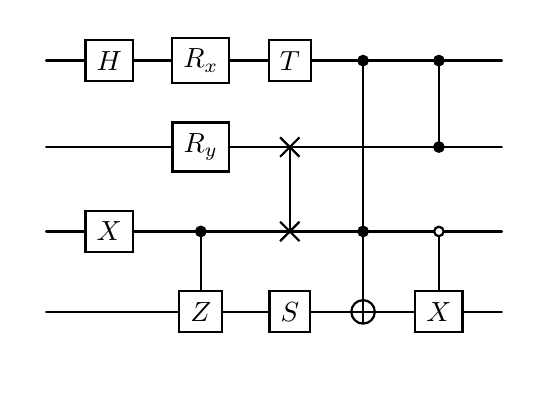
\begin{tikzpicture}[every node/.append style={transform shape}]
            \node{\begin{quantikz}
                & \gate{H} & \gate{R_x} & \gate{T} & \ctrl{2} & \ctrl{1}       & \\
                &          & \gate{R_y} & \swap{1} &          & \control{}     & \\
                & \gate{X} & \ctrl{1}   & \targX{} & \ctrl{1} & \ctrl[open]{1} & \\
                &          & \gate{Z}   & \gate{S} & \targ{}  & \gate{X}       & \\
            \end{quantikz}};
        \end{tikzpicture}
    \end{adjustbox}
\end{figure*}

\end{document}
